\documentclass[border=10pt,margin=5pt,tikz,dvisvgm,rgb,utf8]{standalone}
\usepackage{ctex,xeCJK}  % 中文环境
\setCJKmainfont[BoldFont=Source Han Sans SC]{Source Han Serif SC}
\usepackage{calc,fontawesome,forest,smartdiagram,xcolor}
\usetikzlibrary{animations,arrows,automata,graphs,matrix,positioning,shadows,shapes}

\begin{document}
\renewcommand{\baselinestretch}{0.4}

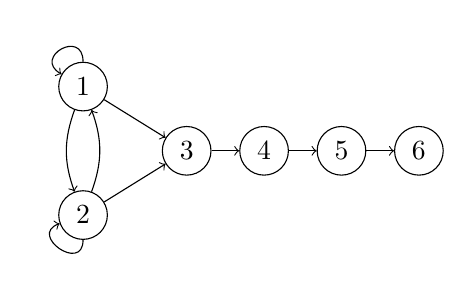
\begin{tikzpicture}
  \node[circle, draw=black](1){1};
  \node[circle, draw=black, below=of 1](2){2};
  \node[circle, draw=black, right=of $(1)!0.5!(2)$](3){3};
  \node[circle, draw=black, right=1em of 3](4){4};
  \node[circle, draw=black, right=1em of 4](5){5};
  \node[circle, draw=black, right=1em of 5](6){6};

  \path[->]
  (1) edge (3)
  (2) edge (3)
  (3) edge (4)
  (4) edge (5)
  (5) edge (6);

  \path[->]
  (1) edge[out=90, in=150, min distance=1.21em] (1)
  (1) edge[out=250, in=110] (2)
  (2) edge[out=270, in=200, min distance=1.21em] (2)
  (2) edge[out=70, in=290] (1);

\end{tikzpicture}

\end{document}
